\documentclass[12pt]{extarticle}
\usepackage[utf8]{inputenc}
\usepackage{cite}
\documentclass{article}
\usepackage{graphicx}
\usepackage[T1]{fontenc}
\usepackage[table,xcdraw]{xcolor}
\usepackage{multirow}
\usepackage{tabularx}


\title{CSE 574 - Intro to Machine Learning - Project 1 Report}
\author{Group 13 - Chaitanya Pawa, Krina Joshi, Vineel Patnana}
\date{March 2019}

\begin{document}

\maketitle

\section{Problem 1 - Gaussian Discriminators}

Linear Discriminant Analysis(LDA) and Quadratic discriminant analysis (QDA) are using the sample training data (sample train) from the sample.pickle file. The accuracy of LDA and QDA on the provided test data set (sample test) is 97\% and 97\% respectively. Below is the  plot of the discriminating boundary for linear and quadratic discriminators along with the points.

\begin{center}
  \centering
  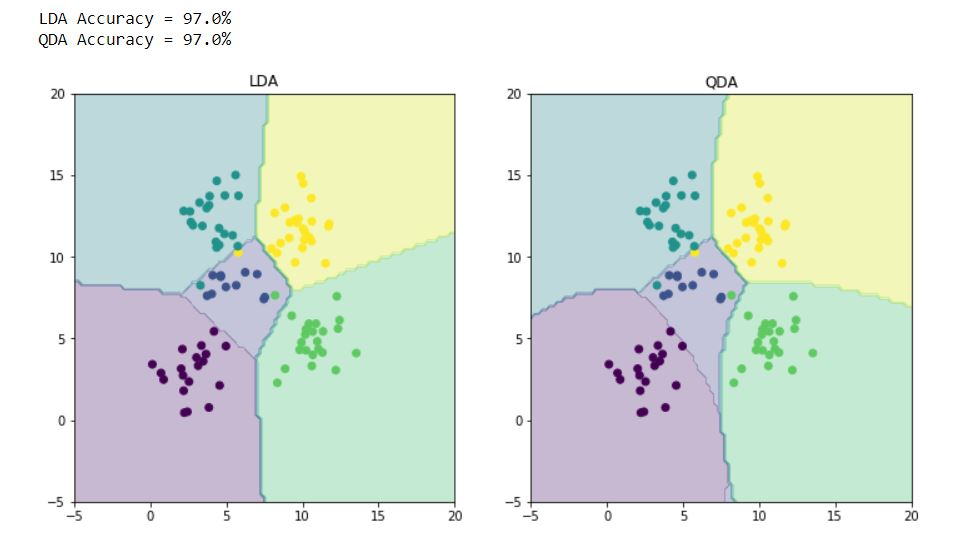
\includegraphics[width=\textwidth]{Q1.JPG}
  \caption{LDA and QDA boundaries along with the points}
\end{center}

\textbf{Inference} - The boundaries for LDA is linear where as that of QDA is quadratic in nature which can be seen from the above plot. 


\begin{center}
  \centering
  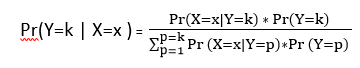
\includegraphics[width=\textwidth]{Bayes_v3.png}
  \caption{Using Bayes theorem to calculate the likelihood}
\end{center}

\newline
\textbf{Pr(Y = k|X = x)} –> Probability that an observation belongs to response class Y = k, provided X = x. (Posterior) 

\textbf{Pr(X = x|Y = k)} –> Probability of X = x, for a particular response class Y = k. (Likelihood)

\vspace{3 mm}
The likelihood is obtained using a Gaussian distribution for both LDA and QDA given by the below equation:

\vspace{3 mm}

{\huge \textbf{${\displaystyle (2\pi )^{-{\frac {k}{2}}}\operatorname {det} ({\boldsymbol {\Sigma }})^{-{\frac {1}{2}}}\,e^{-{\frac {1}{2}}(\mathbf {x} -{\boldsymbol {\mu }})'{\boldsymbol {\Sigma }}^{-1}(\mathbf {x} -{\boldsymbol {\mu }})}}$}}

\vspace{5 mm}
We observe quadratic boundaries in QDA because the covariance matrices  in mahalanobis distance in the probability distribution of likelihood vary for all the 5 classes(${\boldsymbol {\Sigma_1 }},{\boldsymbol {\Sigma_2 }},{\boldsymbol {\Sigma_3 }},{\boldsymbol {\Sigma_4 }},{\boldsymbol {\Sigma_5 }}$) giving rise to higher variation in the quadratic terms and hence quadratic boundaries in the plot. However, in LDA we have the same covariance matrix(${\boldsymbol {\Sigma }}$) for all the 5 classes which has very less variation in the  quadratic terms giving rise to linear terms and hence the linear boundary.

\newpage
\section{Problem 2 - Linear Regression}

Implemented the ordinary least squares method to estimate regression parameters by minimizing the squared loss to find the weights {\boldsymbol  w } as below:

${\displaystyle {\boldsymbol  w }=(X^{T}X)^{-1}X^{T}{\boldsymbol {y}}.}$

\vspace{3 mm}
Above table contains Mean Square Error(MSE) for the training and test data without using an Intercept and with using an intercept.

\vspace{5mm}
\begin{tabularx}{\textwidth}{|X|c|c|}
\hline
\rowcolor[HTML]{FFCE93} 
Model & Training Error & Testing Error \\ \hline
Without Intercept & 19099.44 & 106775.36 \\ \hline
With Intercept & 2187.16 & 3707.84 \\ \hline
\end{tabularx}


\vspace{5mm}
From the above obtained results one can say that, Mean Square Error with Intercept are less for both Training and Test Dataset compared to that of Without Intercept.

\vspace{3mm}
\textbf{Inference} - Without the intercept, obtained regression line will pass through the origin, thereby giving less accurate fit (higher MSE) to all the points. We add bias(intercept) to adjust the slope of the regression line so that it passes through the points more accurately. If you remove the intercept term form the model then the estimate for the slope will change in Regression. Hence, by adding the Intercept term in the model , we make the regression line fit better(lesser MSE), in both train and test set.

\newpage
\section{Problem 3 - Ridge Regression}

Implemented the Ridge Regression on training and test diabetes dataset with different values of $\lambda$ ranging from 0 (no regularization) to 1 in steps of 0.01. 

\vspace{3 mm}
The weights for Ridge Regression are found by adding OLS Loss with an L2 norm penalty and finding the least value of w :
${\boldsymbol  w } = (X^TX + \lambda I)^{-1}X^Ty$

\begin{center}
  \centering
  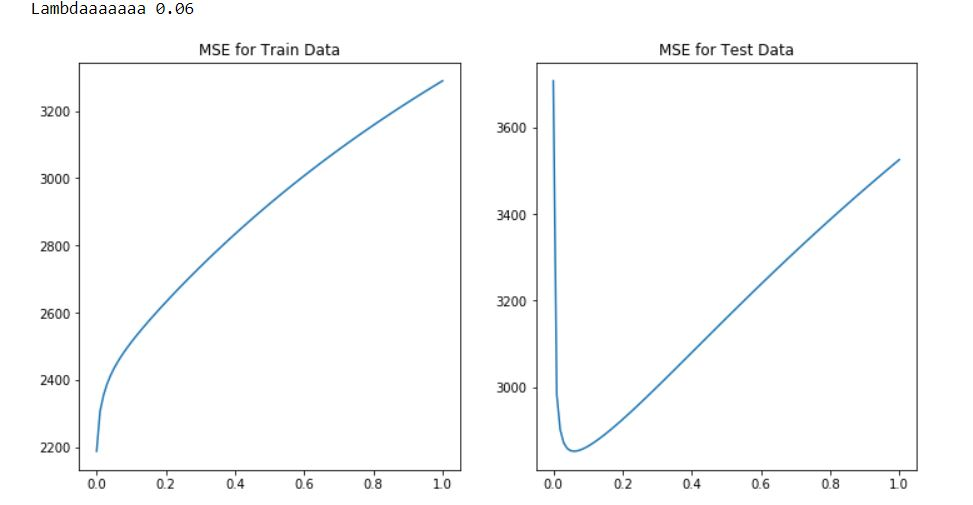
\includegraphics[width=\textwidth]{Q3.JPG}
  \caption{Mean Square Error for Train and Test data vs Lambda Values (Between 0 and 1)}
\end{center}

\textbf{Inference -} By plotting the MSE for train and test data for different values of $\lambda$, we can see from the below plots that minimum test error is obtained when $\lambda$ is very close to 0.06 and hence we can use this for calculating the exact weights better than other $\lambda$ values.

\begin{center}
  \centering
  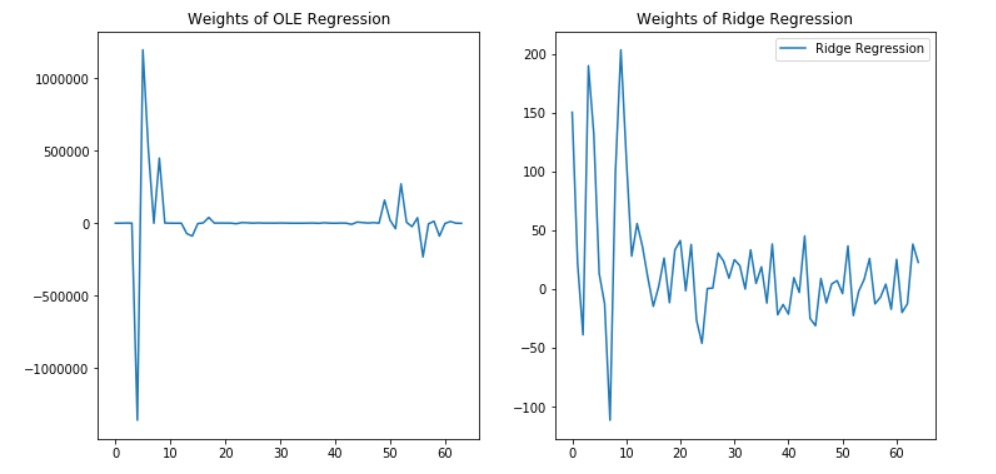
\includegraphics[width=\textwidth]{Q3_2.jpeg}
  \caption{Magnitude of weights for Ridge Regression(Lambda = 0.06) and OLE Regression for all 64 features in the diabetes dataset }
\end{center}

\begin{center}
  \centering
  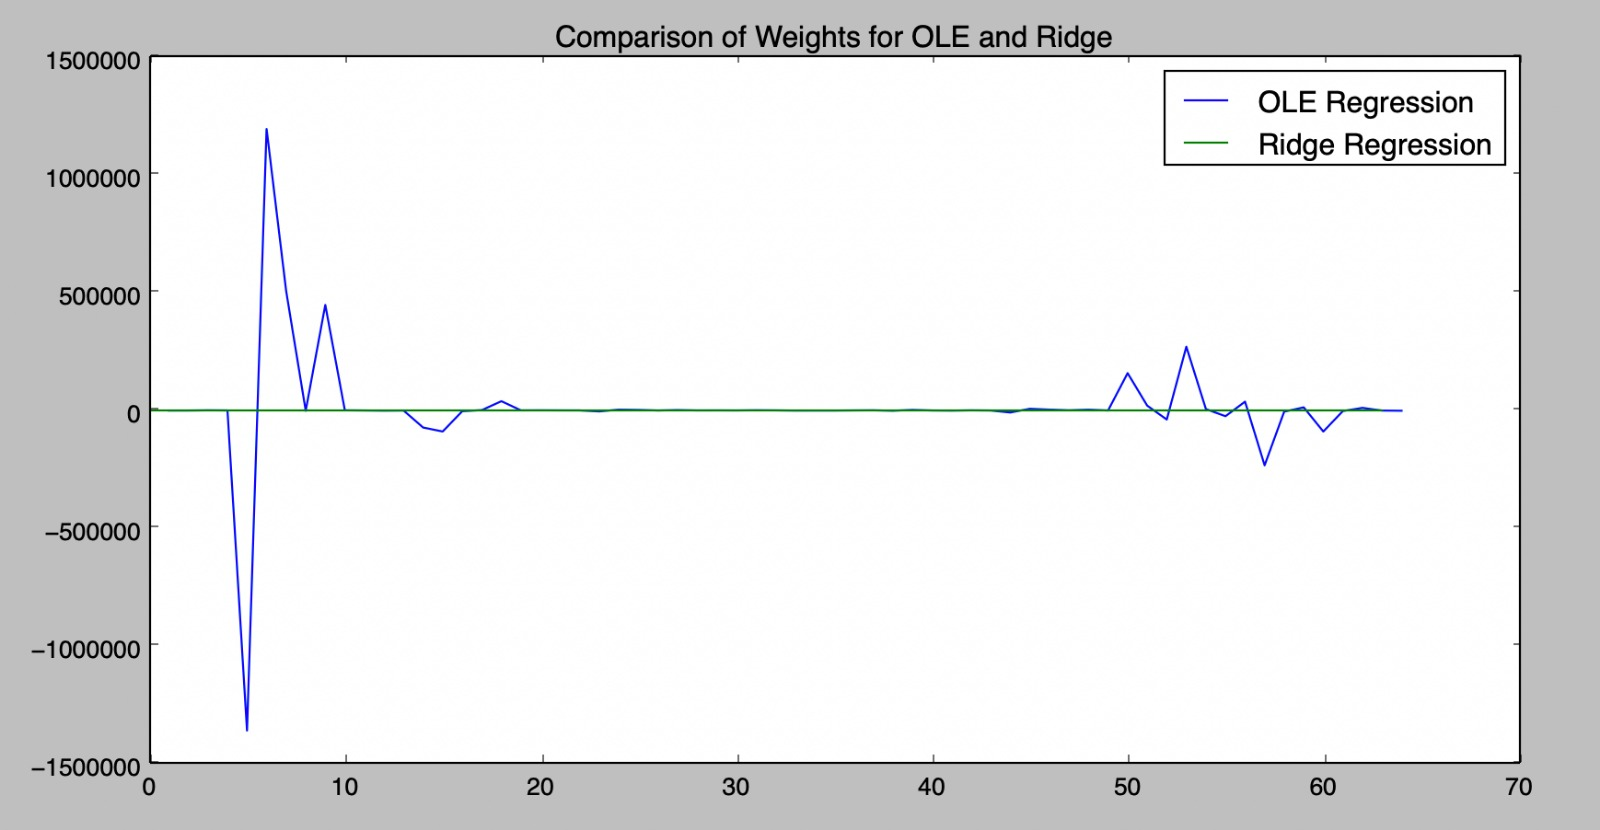
\includegraphics[width=\textwidth]{Q3_1.jpeg}
  \caption{Comparison of magnitude of weights for Ridge Regression(Lambda = 0.06) and OLE Regression for all 64 features in the diabetes dataset }
\end{center}

From the above plots we can see how the weights are varying for OLE and Ridge Regression. The range of weights for OLE is very high compared to that of Ridge Regression as expected due to the regularization. On plotting both of them in one we observe the variation in Ridge Regression is negligible compared to OLE Regression.


\begin{table}[]
\centering
\begin{tabular}{|c|l|c|}
\hline
\rowcolor[HTML]{FFCE93} 
Model & Training Error & Testing Error \\ \hline
Ridge Regression($\lambda$ = 0.06) & 2451.53 & 2851.33 \\ \hline
OLE Regression with Intercept & 2187.16 & 3707.84 \\ \hline
\end{tabular}
\end{table}

\vspace{3mm}
The table shows the comparison of Training and Test error in Ridge and OLE Regression with Intercept. The Training error is lesser for OLE Regression but as expected the testing error is less for Ridge Regression as it doesn't overfit and it generalizes better than an OLE Regression.

\newpage
\section{Problem 4 - Gradient Descent for Ridge Regression Learning}

We implemented the gradient descent procedure for estimating the weights - ‘w’ by varying the different values of lambda (regularizing parameter). The Train MSE and the Test MSE for different values of Lambda are plotted below.

\begin{center}
  \centering
  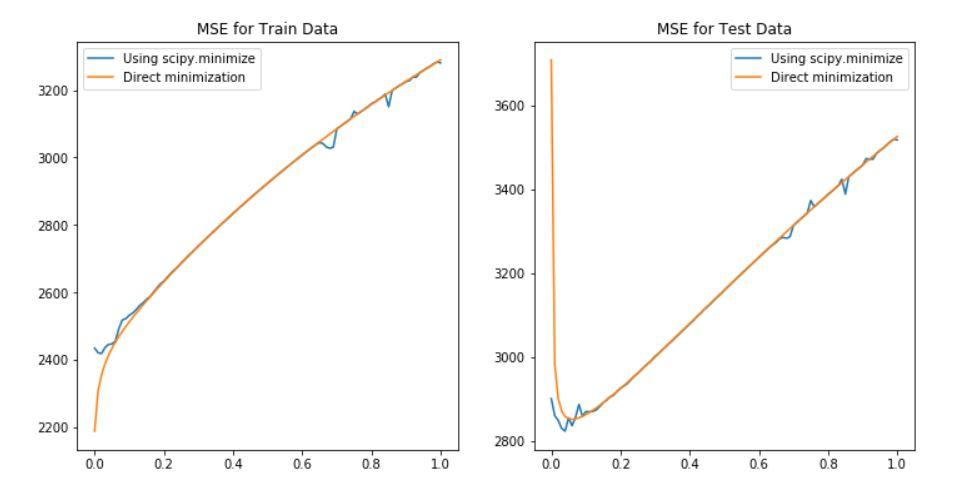
\includegraphics[width=\textwidth]{Q4.JPG}
  \caption{Mean Square Error for Train and Test data vs Lambda Values for Ridge Regression using Ordinary Least Squares(Orange) and Gradient Descent(Blue)}
\end{center}

\textbf{Inference -}To avoid computation of $(X^TX + \lambda I)^{-1}$ which might not be always defined due to singularity, we use gradient descent to minimize the loss function (or to maximize the log-likelihood) function. 


When Ordinary Least squares is used for Ridge Regression , we got minimum Test error when the value of the regularization parameter $\lambda$ was 0.06.
When gradient descent is used , minimum test error is obtained when $\lambda$ is 0.04. We can see that the error curve for the gradient descent is not smooth at $\lambda$ = 0.04, which can be due to the anomaly(outliers) in the data and also because of the way gradient descent works with respect to the learning rate we can see oscillations as compared to the OLS. We might get slightly overfitted model when gradient descent is used.

\newpage
\section{Problem 5 - Non-linear Regression}

The errors on train and test data for both the values of $\lambda$ is as follows:
\newline

\vspace{5mm}
\begin{tabularx}{\textwidth}{|X|l|l|l|l|}
\hline
\rowcolor[HTML]{FFCE93} 
P & Train ($\lambda$ = 0) & Train ($\lambda$ = 0.06)&Test ($\lambda$ = 0)&Test ($\lambda$ = 0.06) \\ \hline

0 & 5650.71&5650.71&6286.40 &6286.87\\ \hline
1  & 3930.91 & 3951.22 & 3845.03 & 3894.70\\ \hline
2& 3911.83 & 3950.05 & 3907.12 & 3894.44\\ \hline
3 & 3911.18 & 3950.05 & 3887.97 & 3894.44\\ \hline
4 & 3885.47 & 3950.05 & 4443.32 & 3894.44\\ \hline
5 & 3885.40 & 3950.05 & 4554.83 & 3894.44\\ \hline
6 & 3866.88&3950.05 & 6833.45 & 3894.44\\ \hline

\end{tabularx}

\vspace{5mm}
The optimal value for p when $\lambda$ = 0 is 1 as the minimum testing error (3845.03) is observed at this value of p. When p=1, the model is nothing but linear ridge regression. Thus we can infer that linear ridge regression is actually the optimal method for better generalization.

\newline
The optimal value for p when $\lambda$ = 0.06 is 1 as the minimum testing error (3894.70) is observed at this value of p. 

Plotting the curve for the optimal value of p for both values of $\lambda$, we get the following curves.

\begin{center}
  \centering
  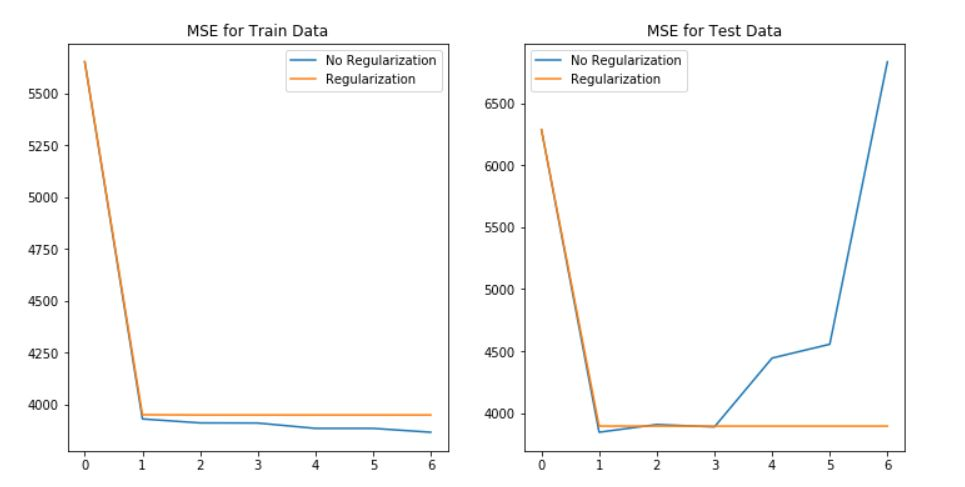
\includegraphics[width=\textwidth]{Q5.JPG}
  \caption{MSE for Train and Test for different value of p }
\end{center}

From the above plots, we can infer that in the event of no regularization, the training error keeps on decreasing as the order of the polynomial increases whereas the testing error decreases at first and then increases sharply. This is due to the over-fitting of the model on the training data. As the degree increases the model fits the training data very well, but in the case of the test data it is not able to generalize well and thus we see such a sharp increase in the test error.


\vspace{3mm}
In the event of regularization, we see that the training error decreases at first but then becomes close to a constant value. It means that the model achieves an optimal state at a low p value and thus the training error does not decrease further in turn avoiding over-fitting. In the case of test data, we can see that the test error also reaches an optimal value for p = 1 as it becomes almost constant for values of p from 1 to 6. 

\newpage
\section{Problem 6 - Interpreting the Results }

Training and Test Error for different models are shown in the below table:

\vspace{5 mm}
\begin{tabularx}{\textwidth}{|X|c|c|}
\rowcolor[HTML]{FFCE93}
\hline
Model & Min Training Error & Min Testing Error \\ \hline

OLE Regression with Intercept & 2187.16 &3707.84 \\ \hline
OLE Regression without Intercept & 19099.44& 106775.36\\ \hline
Ridge Regression(Lambda = 0.06) &2451.52& 2851.33\\ \hline
Ridge Regression Using Gradient Descent (Lambda = 0.04) &2463.05&2853.50\\ \hline
Regression with higher order polynomial (with Regularization) &3950.05 for p=6 &3894.44 for p=3\\ \hline
Regression with higher order polynomial(without Regularization) &3866.88  for p= 6 &3845.03 for p=1 \\ \hline
\end{tabularx}

\vspace{5mm}
Test Error in increasing order: 
\textbf{Ridge Regression < Ridge Regression Using Gradient Descent < OLE Regression with Intercept < Regression with higher order polynomial(without Regularization) < Regression with higher order polynomial (with Regularization) < OLE Regression without Intercept}

\vspace{3mm}
\textbf{Inference-} To make final recommendations for anyone using regression for predicting diabetes level using the input features one can use Ridge Regression

One can observe that the model with best prediction is Ridge Regression which is also giving the least generalization Training and Testing error, as compared to all other implemented models. Regression using higher order polynomials give poor generalization error as it will overfit.

\vspace{3mm}
Consider the case of Regression with higher order polynomial, with degree 6, although it will fit the training set better it leads to overfitting and hence will not give good test errors. Hence,\textbf{ Least Test error} should be considered as the metric to choose the best model.

\vspace{3mm}
Thus we can say that the linear ridge regression is the best when it comes to making a generalized prediction model. It avoids the over-fitting as well as does a good job at regularization.
\end{document}
